% questions.tex —— 2001 年·春季上海卷 · 题目内容片段（无答案）
% 由 tools/generate_projects.py 依来源总账自 2001/2001_数学真题_春季上海_试题.md 生成，勿手改（改源 MD 后重跑）


\gkpart{数学}

\begin{gktip}
\textbf{来源说明}：本题面依据固定源 PDF《2001 普通高等学校春季招生考试（上海卷）》两页题面逐题转录，原卷印刷页码 83–84。固定源不附答案，答案和解析均由本库独立复算。

\textbf{图形说明}：第 19、20 题的原卷图形关系重绘为 TikZ/PGFPlots 矢量图。图形标记所指的 PNG 不随仓库保存。
\end{gktip}

\gkpart{一、填空题}

\begin{question}
\gkti{1}函数 $f(x)=x^2+1$（$x\le0$）的反函数 $f^{-1}(x)=$\gkblank{}。

\end{question}
\begin{question}
\gkti{2}若复数 $z$ 满足方程 $zi=i-1$（$i$ 是虚数单位），则 $z=$\gkblank{}。

\end{question}
\begin{question}
\gkti{3}函数

\nopagebreak[4]
\[
y=\dfrac{\sin x}{1-\cos x}
\]

的最小正周期为\gkblank{}。

\end{question}
\begin{question}
\gkti{4}二项式

\nopagebreak[4]
\[
\left(x+\dfrac1x\right)^6
\]

的展开式中常数项的值为\gkblank{}。

\end{question}
\begin{question}
\gkti{5}若双曲线的一个顶点坐标为 $(3,0)$，焦距为 $10$，则它的标准方程为\gkblank{}。

\end{question}
\begin{question}
\gkti{6}圆心在直线 $y=x$ 上且与 $x$ 轴相切于点 $(1,0)$ 的圆的方程为\gkblank{}。

\end{question}
\begin{question}
\gkti{7}计算

\nopagebreak[4]
\[
\lim_{n\to\infty}\left(\dfrac{n+3}{n+1}\right)^n
\]

。

\end{question}
\begin{question}
\gkti{8}若向量 $\boldsymbol{\alpha}$、$\boldsymbol{\beta}$ 满足 $\lvert\boldsymbol{\alpha}+\boldsymbol{\beta}\rvert=\lvert\boldsymbol{\alpha}-\boldsymbol{\beta}\rvert$，则 $\boldsymbol{\alpha}$ 与 $\boldsymbol{\beta}$ 所成角的大小为\gkblank{}。

\end{question}
\begin{question}
\gkti{9}在大小相同的 $6$ 个球中，$2$ 个红球，$4$ 个是白球。若从中任意选取 $3$ 个，则所选的 $3$ 个球中至少有 $1$ 个红球的概率是\gkblank{}。（结果用分数表示）

\end{question}
\begin{question}
\gkti{10}若记号“$\ast$”表示求两个实数 $a$ 与 $b$ 的算术平均数的运算，即

\nopagebreak[4]
\[
a\ast b=\dfrac{a+b}{2}
\]

则两边均含有运算符号“$\ast$”和“$+$”，且对于任意 $3$ 个实数 $a\text{、}b\text{、}c$ 都能成立的一个等式可以是\gkblank{}。

\end{question}
\begin{question}
\gkti{11}关于 $x$ 的函数 $f(x)=\sin(x+\varphi)$ 有以下命题：

（1）对任意的 $\varphi$，$f(x)$ 都是非奇非偶函数；

（2）不存在 $\varphi$，使 $f(x)$ 既是奇函数，又是偶函数；

（3）存在 $\varphi$，使 $f(x)$ 是奇函数；

（4）对任意的 $\varphi$，$f(x)$ 都不是偶函数。

其中一个假命题的序号是\gkblank{}。因为当 $\varphi=$\gkblank{} 时，该命题的结论不成立。

\end{question}
\begin{question}
\gkti{12}甲、乙两人于同一天分别携款 $1$ 万元到银行储蓄，甲存五年期定期储蓄，年利率为 $2.88\%$。乙存一年期定期储蓄，年利率为 $2.25\%$，并在每年到期时将本息续存一年期定期储蓄。按规定每次计息时，储户须交纳利息的 $20\%$ 作为利息税。若存满五年后两人同时从银行取出存款，则甲与乙所得本息之和的差为\gkblank{}元。（假定利率五年内保持不变，结果精确到 $1$ 分）

\end{question}
\gkpart{二、选择题}

\begin{question}
\gkti{13}若 $a\text{、}b$ 为实数，则 $a>b>0$ 是 $a^2>b^2$ 的\mbox{（　　）}

（A）充分不必要条件　　（B）必要不充分条件

（C）充要条件　　（D）既非充分条件也非必要条件

\end{question}
\begin{question}
\gkti{14}若直线 $x=1$ 的倾斜角为 $\alpha$，则 $\alpha$\mbox{（　　）}

（A）等于 $0$　　（B）等于 $\dfrac\pi4$　　（C）等于 $\dfrac\pi2$　　（D）不存在

\end{question}
\begin{question}
\gkti{15}若有平面 $\alpha$ 与 $\beta$，且 $\alpha\cap\beta=l$，$\alpha\perp\beta$，$P\in\alpha$，$P\notin l$，则下列命题中的假命题为\mbox{（　　）}

（A）过点 $P$ 且垂直于 $\alpha$ 的直线平行于 $\beta$

（B）过点 $P$ 且垂直于 $l$ 的平面垂直于 $\beta$

（C）过点 $P$ 且垂直于 $\beta$ 的直线在 $\alpha$ 内

（D）过点 $P$ 且垂直于 $l$ 的直线在 $\alpha$ 内

\end{question}
\begin{question}
\gkti{16}若数列 $\{a_n\}$ 前 $8$ 项的值各异，且 $a_{n+8}=a_n$ 对任意的 $n\in\mathbb N$ 都成立，则下列数列中可取遍 $\{a_n\}$ 前 $8$ 项值的数列为\mbox{（　　）}

（A）$\{a_{2k+1}\}$　　（B）$\{a_{3k+1}\}$　　（C）$\{a_{4k+1}\}$　　（D）$\{a_{6k+1}\}$

\end{question}
\gkpart{三、解答题}

\begin{question}
\gkti{17}已知 $\mathbb R$ 为全集，

\nopagebreak[4]
\[
A=\left\{x\mid\log_{\frac12}(3-x)\ge-2\right\},\qquad
B=\left\{x\mid\dfrac5{x+2}\ge1\right\}
\]

求 $\overline A\cap B$。

\end{question}
\begin{question}
\gkti{18}已知

\nopagebreak[4]
\[
\dfrac{2\sin^2\alpha+\sin2\alpha}{1+\tan\alpha}=k
\quad\left(\dfrac\pi4<\alpha<\dfrac\pi2\right)
\]

试用 $k$ 表示 $\sin\alpha-\cos\alpha$ 的值。

\Needspace{0.4\textheight}
\end{question}
\begin{question}
\gkti{19}用一块钢锭浇铸一个厚度均匀，且全面积为 $2$ 平方米的正四棱锥形有盖容器（如图），设容器的高为 $h$ 米，盖子边长为 $a$ 米。
\nopagebreak[4]
\begin{center}% 2001 年春季上海卷第 19 题：正四棱锥形有盖容器
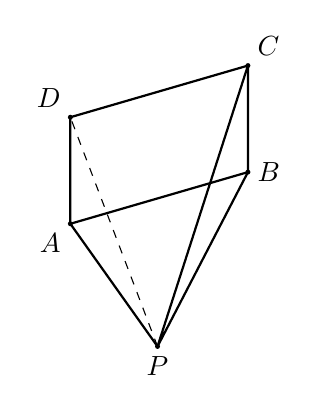
\begin{tikzpicture}[>=stealth, scale=0.82]
  \coordinate (A) at (0,0);
  \coordinate (B) at (2.75,0.8);
  \coordinate (C) at (2.75,2.45);
  \coordinate (D) at (0,1.65);
  \coordinate (P) at (1.35,-1.9);

  \draw[thick] (A)--(B)--(C)--(D)--cycle;
  \draw[thick] (P)--(A) (P)--(B) (P)--(C);
  \draw[dashed] (P)--(D);

  \fill (A) circle (1.1pt) node[below left] {$A$};
  \fill (B) circle (1.1pt) node[right] {$B$};
  \fill (C) circle (1.1pt) node[above right] {$C$};
  \fill (D) circle (1.1pt) node[above left] {$D$};
  \fill (P) circle (1.1pt) node[below] {$P$};
\end{tikzpicture}
\end{center}
\nopagebreak[4]
（1） 求 $a$ 关于 $h$ 的函数解析式；

（2） 设容器的容积为 $V$ 立方米，则当 $h$ 为何值时，$V$ 最大？求出 $V$ 的最大值。

注：求解本题时，不计容器的厚度。

\Needspace{0.4\textheight}
\end{question}
\begin{question}
\gkti{20}在长方体 $ABCD-A_1B_1C_1D_1$ 中，点 $E\text{、}F$ 分别在 $BB_1\text{、}DD_1$ 上，且 $AE\perp A_1B$，$AF\perp A_1D$。
\nopagebreak[4]
\begin{center}% 2001 年春季上海卷第 20 题：长方体中的点与平面
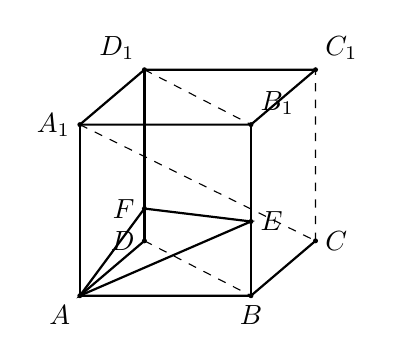
\begin{tikzpicture}[>=stealth, scale=0.82]
  \coordinate (A) at (0,0);
  \coordinate (B) at (2.65,0);
  \coordinate (C) at (3.65,0.85);
  \coordinate (D) at (1,0.85);
  \coordinate (A1) at (0,2.65);
  \coordinate (B1) at (2.65,2.65);
  \coordinate (C1) at (3.65,3.5);
  \coordinate (D1) at (1,3.5);
  \coordinate (E) at (2.65,1.15);
  \coordinate (F) at (1,1.35);

  \draw[thick] (A)--(B)--(C);
  \draw[thick] (A)--(D);
  \draw[thick] (A1)--(B1)--(C1);
  \draw[thick] (A1)--(D1)--(C1);
  \draw[thick] (A)--(A1) (B)--(B1) (D)--(D1);
  \draw[dashed] (C)--(C1) (D1)--(B1) (D)--(B);
  \draw[thick] (A)--(E)--(F)--cycle;
  \draw[dashed] (A1)--(C);

  \fill (A) circle (1.1pt) node[below left] {$A$};
  \fill (B) circle (1.1pt) node[below] {$B$};
  \fill (C) circle (1.1pt) node[right] {$C$};
  \fill (D) circle (1.1pt) node[left] {$D$};
  \fill (A1) circle (1.1pt) node[left] {$A_1$};
  \fill (B1) circle (1.1pt) node[above right] {$B_1$};
  \fill (C1) circle (1.1pt) node[above right] {$C_1$};
  \fill (D1) circle (1.1pt) node[above left] {$D_1$};
  \fill (E) circle (1.1pt) node[right] {$E$};
  \fill (F) circle (1.1pt) node[left] {$F$};
\end{tikzpicture}
\end{center}
\nopagebreak[4]
（1） 求证：$A_1C\perp$ 平面 $AEF$；

（2） 若规定两个平面所成的角是这两个平面所组成的二面角中的锐角（或直角），则在空间中有定理：若两条直线分别垂直于两个平面，则这两条直线所成的角与这两个平面所成的角相等。试根据上述定理，在 $AB=4$，$AD=3$，$AA_1=5$ 时，求平面 $AEF$ 与平面 $D_1B_1BD$ 所成的角的大小。（用反三角函数值表示）

\end{question}
\begin{question}
\gkti{21}已知椭圆 $C$ 的方程为

\nopagebreak[4]
\[
x^2+\dfrac{y^2}{2}=1
\]

\Needspace{5\baselineskip}
点 $P(a,b)$ 的坐标满足

\nopagebreak[4]
\[
a^2+\dfrac{b^2}{2}\le1
\]

过点 $P$ 的直线 $l$ 与椭圆交于 $A\text{、}B$ 两点，点 $Q$ 为线段 $AB$ 的中点，求：

（1） 点 $Q$ 的轨迹方程；

（2） 点 $Q$ 的轨迹与坐标轴的交点的个数。

\end{question}
\begin{question}
\gkti{22}已知 $\{a_n\}$ 是首项为 $2$，公比为 $\dfrac12$ 的等比数列，$S_n$ 为它的前 $n$ 项和。

（1） 用 $S_n$ 表示 $S_{n+1}$；

\Needspace{5\baselineskip}
（2） 是否存在自然数 $c$ 和 $k$，使得

\nopagebreak[4]
\[
\dfrac{S_{k+1}-c}{S_k-c}>2
\]

成立。

\end{question}